

% Language setting
% Replace `english' with e.g. `spanish' to change the document language

\documentclass[11pt]{article}
\usepackage[french]{babel}
\usepackage{wrapfig}
\usepackage{tikz}
\usepackage[a4paper,top=2cm,bottom=2cm,left=3cm,right=3cm,marginparwidth=1.75cm]{geometry}
\usepackage{amsmath}
\usepackage{graphicx}
\usepackage{varwidth}
\usepackage{url}
\usepackage{algorithmic}
\usepackage[french,boxed,ruled,lined]{algorithm2e}
\usepackage{fancyhdr}
\usepackage{algpseudocode}
\usepackage[colorlinks=true, allcolors=blue]{hyperref}
\usepackage[T1]{fontenc} 
\usepackage{xcolor}
\usepackage{listings}
\usepackage{algorithmicx}

\definecolor{codegreen}{rgb}{0,0.6,0}
\definecolor{codegray}{rgb}{0.5,0.5,0.5}
\definecolor{codepurple}{rgb}{0.58,0,0.82}
\definecolor{backcolour}{rgb}{0.95,0.95,0.92}

\lstdefinestyle{mystyle}{
    backgroundcolor=\color{backcolour},   
    commentstyle=\color{codegreen},
    keywordstyle=\color{magenta},
    numberstyle=\tiny\color{codegray},
    stringstyle=\color{codepurple},
    basicstyle=\ttfamily\footnotesize,
    breakatwhitespace=false,         
    breaklines=true,                 
    captionpos=b,                    
    keepspaces=true,                 
    numbers=left,                    
    numbersep=5pt,                  
    showspaces=false,                
    showstringspaces=false,
    showtabs=false,                  
    tabsize=2
}

\lstset{style=mystyle}

\title{ENSEIRB-MATMECA I1\\Rapport de projet d'algorithmique et de programmation n°2  \\
\begin{figure}[h]
\begin{tikzpicture}[scale=1.3]
\draw (0,0) -- (12,0);  
\end{tikzpicture}
\end{figure}
\vspace{1cm}
\textbf{\Huge Amazons}}
\vspace{1cm}

\author{ \\ Abderahim LAGRAOUI \\ Majid MEDGHALI  \\ Moussa ALLOUBANE\\ Mohammed BOUHAJA \\\\\\ \textbf{Encadrant:} DAVID Jean-Francois}
\date{}
\usepackage{fancyhdr}
\pagestyle{fancy}

\renewcommand{\headrulewidth}{1pt}
\fancyhead[]{} 
%\fancyhead[C]{\textbf{page \thepage}} 
%\fancyhead[L]{\leftmark}
%\fancyhead[R]{machin}
\renewcommand{\footrulewidth}{1pt}
\fancyfoot[C]{{\thepage/16}} 
\fancyfoot[L]{Projet de programmation N°2}
\fancyfoot[R]{Année 2022/2023}


\begin{document}
\maketitle
\begin{figure}[h]
    \centering
    
\includegraphics[height = 8cm , width = 14cm]{LOGO_EM.png}
\end{figure}
\newpage
\tableofcontents
    \newpage
    \section{Introduction}
        \subsection{Présentation générale du projet}
            Le Jeu des Amazones est un jeu de société à deux joueurs inventé en 1988 par Walter Zamkauskas. Le jeu se joue sur un plateau carré avec une grille de 10x10 cases. Chaque joueur dispose de quatre pièces, appelées Amazones, qui commencent aux coins opposés du plateau comme le montre la figure~\ref{fig:amazones}. L'objectif du jeu est d'être le dernier joueur à pouvoir faire un mouvement légal.
            Le jeu des Amazones est un jeu complexe et stratégique qui implique une planification minutieuse et une exécution précise.
            \begin{figure}[h]
                \centering
                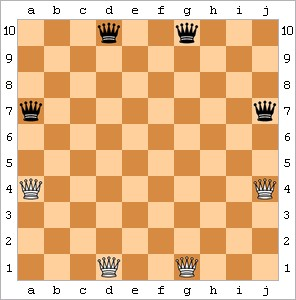
\includegraphics[scale=0.7]{Amazons_starting_position.jpg}
                \caption{Les positions de départ dans le jeu des Amazones}
                \label{fig:amazones}
            \end{figure}
            
        \subsection {Problématique}
             La problématique principale était de comprendre et de faire une abstraction du jeu en appliquant tous les aspects de la programmation impérative, de bien échanger les idées et les connaissances au sein du groupe et de savoir les acheminer pour résoudre les différentes difficultés aux niveaux de compilation, organisation du dépôt et synchronisation des travaux faits par chaque contributeur. 
        \subsection{Difficultés}
            \subsubsection{Implémentation du plateau de jeu}
            L'implémentation du plateau de jeu en utilisant la bibliothèque GSL s'est révélée nécessaire pour permettre la représentation du jeu des amazones sous forme de graphes. Cependant, cela a engendré plusieurs difficultés techniques.

            En plus des problèmes liés à la manipulation des fonctions et champs de la bibliothèque, ainsi que la gestion de la mémoire et le passage du graphe vers la grille du jeu, on a également rencontré des difficultés dans la gestion des mouvements et des règles du jeu. Il a fallu prendre en compte les différentes contraintes et possibilités de déplacement des Amazones, ainsi que les règles de blocage des cases après leur utilisation.

            De plus, l'implémentation d'un système de vérification des coups légaux pour éviter les tricheries a ajouté une complexité supplémentaire à l'ensemble du projet. En somme, l'utilisation de la bibliothèque GSL pour implémenter le plateau de jeu a nécessité des compétences techniques avancées et une compréhension approfondie des règles du jeu des Amazones.
            \subsubsection{Implémentation du serveur}
           L'initialisation des joueurs pour le jeu nécessite la transmission de deux graphes et deux tableaux pour les positions des reines. Cependant, cette méthode pose des problèmes liés à la gestion des copies des graphes et des positions initiales. Dans un premier temps, nous avons utilisé le même tableau pour les positions des reines pour les deux joueurs, ce qui a créé un problème lors de la libération de la mémoire. En effet, les deux joueurs tentaient de libérer le même tableau, ce qui provoquait une double libération. De plus, cela permettait à chaque joueur de modifier les positions de l'autre, ce qui n'était pas souhaitable. Ce problème est similaire au fait de ne pas pouvoir utiliser le même joueur deux fois lors d'une partie. Par ailleurs, les joueurs tentaient de libérer un seul graphe et un seul tableau de positions initiales, alors que le serveur en créait deux. Pour éviter ces problèmes, il est recommandé de fournir à chaque joueur un graphe et un tableau de positions de reines distincts pour éviter les conflits lors de la libération de la mémoire et empêcher les joueurs de modifier les positions de l'autre joueur.


        
        \subsection{Architecture du projet}
            Le projet en question est composé d'un ensemble de fichiers écrits en langage de programmation C. Afin de compiler le projet, l'outil Makefile est utilisé, comportant trois règles principales, à savoir $libraries$ pour  générer les bibliothèques partagées de chaque client, $install$ pour compiler l'ensemble des fichiers sources et les copier les éléments nécessaires dans l'emplacement $install/$ et $test$ pour compiler les fichiers de tests et mesurer leur couverture. 
            
            Pour organiser les travaux, l'outil Git est employé, qui permet de travailler sur une version centrale tout en synchronisant les sources. En ce qui concerne la modularité, la figure~\ref{graphe de dépendances} illustre le graphe de dépendances des entêtes des fichiers sources de ce projet sauf qu'il ne suffit pas pour décrire pour l'ensemble des dépendances. En effet, de nombreux fichiers, notamment ceux relatifs aux tests, recourent à des références externes pour chercher les symboles manquants, ce qui ne se reflète pas dans ledit graphe.
    \begin{figure}[h]
        \centering
        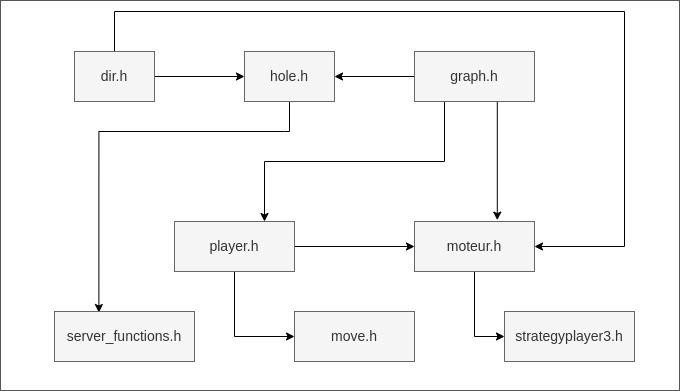
\includegraphics[height = 6.5cm, width = 12.5cm]{graph_dpendances_c (4).jpg}
        \caption{Graphe de dépendances}
        \label{graphe de dépendances}
    \end{figure}
    \section{Définition du monde }
        Cette section s'intéresse à introduire les caractéristiques du monde dans le cadre de son abstraction.
        \subsection{Tableau du jeu}
        Le tableau du jeu est une grille en 2D de taille variable $m > 4$, ses principaux éléments sont les reines qui peuvent se déplacer suivant les mêmes règles des jeux d'échecs, en envoyant une flèche après chaque déplacement avec chaque case peut être vide ou occupée par une amazone ou une flèche. En plus de la grille de jeu de base, les parties peuvent être jouées sur plusieurs types de mondes ou graphes, ce qui peut modifier les règles et les stratégies du jeu. Ces variations incluent des mondes en donut, en trèfle et en huit, qui offrent chacun des configurations différentes pour la grille de jeu et les mouvements des reines. 
        \subsection{Relations définies sur le monde}
        Puisque chaque reine a une dynamique de mouvement, il faut absolument mettre en
    évidence les relations que maintient chaque position de la grille avec ses voisins. Dans le modèle de base du jeu, selon sa disposition dans la grille, chaque position a un nombre de voisins qui varie entre 3 et 8 voisins dans les 8 directions cardinaux et non cardinaux. De plus, chaque position peut être occupée par au plus une seule reine ou une flèche. Les relations du monde sont implémentées en utilisant la structure de données des graphes dont les sommets sont toutes les positions de la grille.
        \subsection{Utilisation de la bibliothèque GSL}
Au début du projet, on a utilisé les matrices au format c00, bien que la transition vers le format  CSR (Compressed Sparse Row) nous ait permis de réduire considérablement la quantité de mémoire requise pour stocker nos matrices creuses, il faut noter l'inconvénient qu'est la difficulté d'ajouter ou de supprimer des éléments, Comme le format CSR ne stocke que les éléments non nuls de la matrice et les indices de colonnes correspondants dans des tableaux à une dimension, l'ajout ou la suppression d'éléments peut nécessiter la réorganisation de ces tableaux.

        
    \section{Construction du jeu}
    Suite à la discussion générale du sujet dans la section précédente, il est maintenant temps de procéder à une analyse plus détaillée de l'implémentation du jeu.
        \subsection{Définition des structures de données}
         La précision des types abstraits est un élément crucial dans un projet, car elle permet de matérialiser les idées et de maintenir la corrélation entre les concepts abstraits du jeu et les algorithmes nécessaires pour les implémenter, donc elle  assure une compréhension claire et uniforme de la structure de données et de la logique du code.
        \subsubsection{Structure \textbf{graph\_t}}
Le fichier \textit{graph.h} fournit une structure de données appelée \textit{struct graph\_t}, qui est utilisée dans le projet pour manipuler une matrice creuse. Cette matrice représente un graph d'adjacence utilisé pour stocker les relations entre les différentes cases d'une grille. La structure \textit{struct graph\_t} contient un entier \textit{num\_vertices} qui représente le nombre de sommets dans le graph, et un pointeur $t$ vers une matrice creuse de taille "n*n". Les valeurs de la matrice $t$ peuvent être interprétées de la manière suivante : si $t[i][j] > 0$ , cela signifie qu'il existe un arc reliant le sommet i au sommet j dans le graph. De plus, la valeur de $t[i][j]$ permet de désigner une direction.

\begin{lstlisting}[language=C]
struct graph_t {
  unsigned int num_vertices; // Number of vertices in the graph
  gsl_spmatrix_uint* t;      // Sparse matrix of size n*n,
                      // t[i][j] > 0 means there is an edge from i to j
                      // t[i][j] == DIR_NORTH means that j is NORTH of i
                      // t[i][j] == DIR_SOUTH means that j is SOUTH of i
                      // and so on
};
\end{lstlisting}


        
        \subsubsection{Structure \textbf{player\_t}}

        La deuxième structure est la structure \textit{player\_t}, elle est définie dans le fichier \textit{player.h} et est utilisée pour représenter un joueur dans le jeu. Elle contient un identifiant unique, un nom, un pointeur vers un \textit{graph\_t} pour stocker le graphe d'adjacence de ce joueur, un nombre de reines actuelles et des tableaux pour stocker leurs positions, ainsi qu'un compteur de tour pour suivre le déroulement du jeu.
        
\begin{lstlisting}[language=C]
struct player_t {
    unsigned int id;
    char const* name;
    struct graph_t* graph;
    unsigned int num_queens;
    unsigned int* current_queens;
    unsigned int* other_queens;
    unsigned int turn;
};

\end{lstlisting}

        \subsection{Initialisation des relations dans la grille}
            Suite à la définition des structures de données, il est désormais possible de initialiser les relations entre les positions de la grille.
            \subsubsection{Initialisation des joueurs}
           Chaque joueur est initialisé en appelant la fonction \textit{initialize} avec en paramètres un graphe ainsi qu'une copie des positions initiales des reines. Cette initialisation se fait en créant un graphe pour le joueur, puis en définissant ses positions initiales de ses reines \textit{current\_positions} ainsi que les positions initiales des reines de son adversaire \textit{other\_positions}. Cette initialisation se fait en utilisant l'allocation dynamique de la mémoire.
            \subsubsection{Initialisation des graphes}
            Pour initialiser un graphe, on implémente une fonction \textbf{initialize\_graph} qui prend en paramètre un entier représentant la taille souhaitée du graphe. La fonction s'en charge d'allouer l'espace mémoire en utilisant les fonctions de GSL et initialise les relations entre tous les sommets. Enfin, comme cette fonction est conçue pour utiliser le format de ligne compressée \textit{CSR}, elle compresse la matrice d'adjacence créée en utilisant la fonction \textbf{gsl\_spmatrix\_uint\_compress} avant de renvoyer un pointeur vers le graphe initialisé. Le graphe crée ainsi est un graphe carré dont tous les sommets sont jouables. Cependant, les autres formes de graphes décrites dans la section suivante nécessite d'isoler un nombre de sommets.

        \subsection{Mise en oeuvre des 4 formes de graphes}
        Le jeu présente plusieurs variantes de tableaux de jeu, il s'agit de 4 formes différentes de graphes dépendants chacun de sa taille, en assurant la symétrie des positions initiales des deux joueurs. 
            \subsubsection{Graphe carré}
            Le graphe carré, c'est le graphe du jeu par défaut, comme le montre la figure~\ref{fig:graphc}, il est constitué de $m^{2}$ sommets tous jouables avec $m$ sa longueur. Le nombre de reines pour chaque joueur varie en fonction de la taille et il a pour valeur $m = 4\times(\frac{m}{10} + 1)$
            \begin{figure}[h]
                \centering
                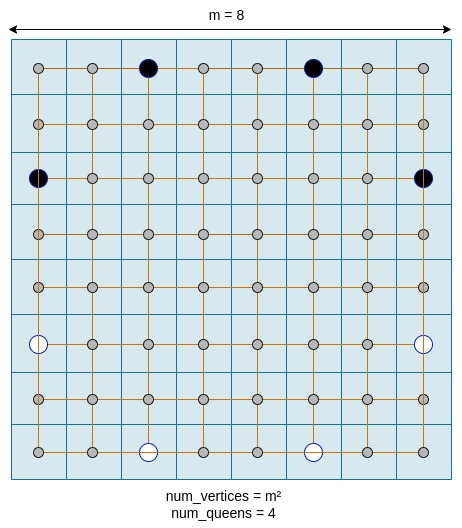
\includegraphics[width = 8cm, height = 8cm]{graphe_carre (3).jpg}
                \caption{Graphe carré}
                \label{fig:graphc}
            \end{figure}
            \newpage
            \subsubsection{Graphe donut}
            Le graphe de type "donut" possède une dimension, notée m, qui est un multiple de trois. Sa particularité réside dans la présence d'un trou central de dimension m/3. La méthode pour sa construction consiste à diviser le graphe en trois blocs verticaux et trois blocs horizontaux, chacun de dimension m/3 comme l'indique la figure~\ref{fig:graphd}. Les sommets correspondant à la zone d'intersection des deux blocs centraux sont isolés, garantissant ainsi la création d'un trou centré précisément au milieu du graphe. Le nombre total de sommets est $8\times \frac{m^{2}}{9}$.
            \begin{figure}[h]
                \centering
                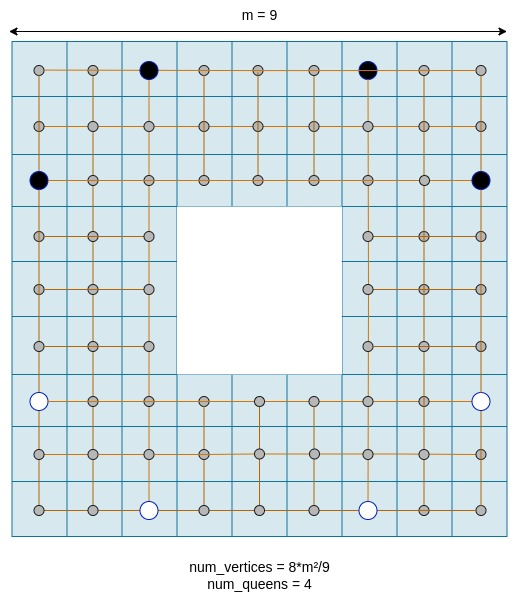
\includegraphics[width = 9cm, height = 8.5cm]{graphe_donut (1).jpg}
                \caption{Graphe donut}
                \label{fig:graphd}
            \end{figure}
            \subsubsection{Graphe trèfle}
            Le graphe en forme de "trèfle" a une dimension, appelée m, qui est un multiple de 5. Sa particularité est qu'il possède 4 trous de taille m/5. Pour le construire, on suit une méthode similaire à celle du graphe en forme de "donut", mais cette fois-ci, on isole 4 carrés pour créer les trous de taille m/5. En isolant ces sommets, on obtient un graphe qui ressemble à celui montré dans la figure~\ref{fig:grapht}. Le nombre total de sommets est $21\times \frac{m^{2}}{5}$.
            \begin{figure}[h]
                \centering
                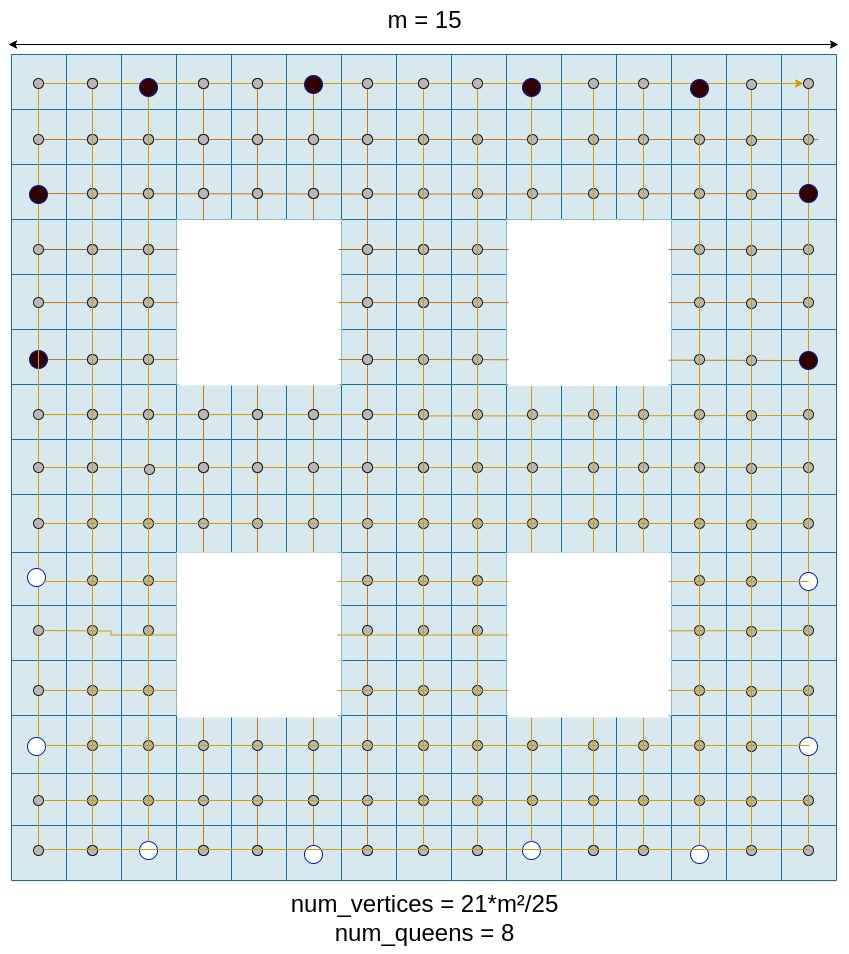
\includegraphics[width = 8.5cm, height = 8cm]{graphe_trefle (2).jpg}
                \caption{graphe trèfle}
                \label{fig:grapht}
            \end{figure}
            \subsubsection{Graphe en huit}
           Le graphe de ce type a une taille m qui est un multiple de 4. Pour le construire, on utilise la même méthode que pour les autres graphes, mais en isolant deux carrés de taille m/4. Cela donne un graphe similaire à celui représenté dans la figure~\ref{fig:graph8}, où la connexion entre les deux sommets centraux est maintenue, comme indiqué sur la même figure. Le nombre total de sommets est $7\times \frac{m^{2}}{8}$.
            \begin{figure}[h]
                \centering
                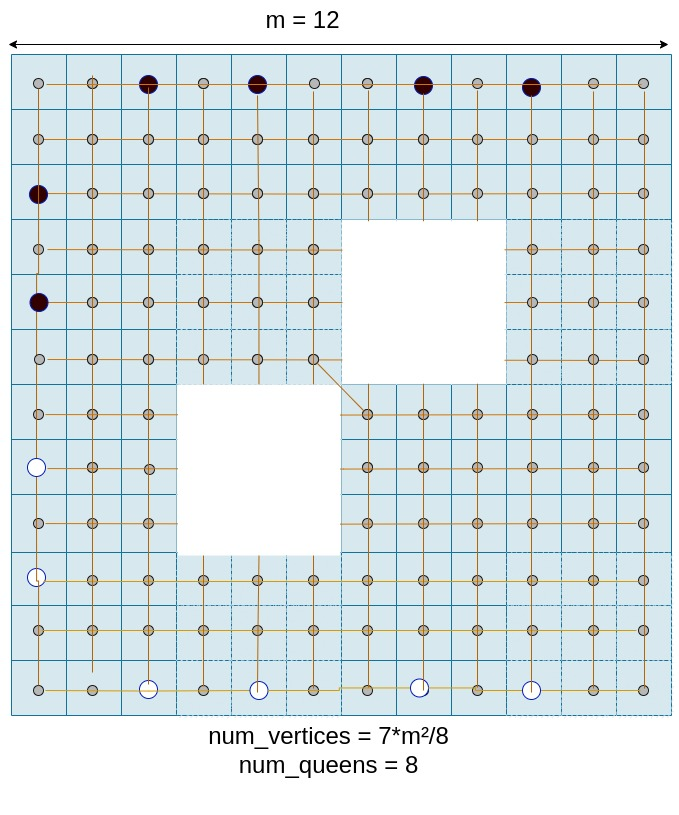
\includegraphics[width = 7cm, height = 7.5cm]{graphe_en8 (3).jpg}
                \caption{Graphe en 8}
                \label{fig:graph8}
            \end{figure}
            \newpage
        \subsection{Communication serveur et client}
        Le serveur a pour mission d'organiser une partie entre deux joueurs en fonction des options choisies. Pour cela, il est nécessaire qu'il initialise les positions de départ et qu'il crée deux copies de ces positions, ainsi que deux copies du graphe pour les deux clients. Les joueurs jouent ensuite tour à tour, et le serveur envoie les coups joués par l'adversaire à chaque joueur. Le serveur est alors chargé de mettre à jour son graphe de jeu à chaque tour avant de passer le coup au joueur suivant. De plus, le serveur doit également informer les clients de la fin de la partie.
        \subsection{Déplacement des reines}
        Les reines peuvent se déplacer horizontalement, verticalement ou en diagonale sur un nombre quelconque de cases vides, à condition qu'elles ne sautent pas par-dessus une autre pièce, ce principe est illustré sur la figure~\ref{fig:deplacments possibles}. 
        
        Après leur déplacement, les reines peuvent lancer une flèche dans n'importe quelle direction (horizontale, verticale ou diagonale) sur un nombre quelconque de cases vides. La case où la flèche est lancée doit être dans la même direction que le déplacement de la reine et doit être située à une distance d'au moins une case de la reine. La flèche se déplace ensuite jusqu'à rencontrer une pièce ou le bord du plateau comme le montre la figure~\ref{fig:fleches possibilites}. Les reines ne peuvent pas se déplacer ni lancer une flèche à travers une case occupée.
                    \begin{figure}[h]
                \begin{minipage}[c]{.45\linewidth}
                    \centering
                    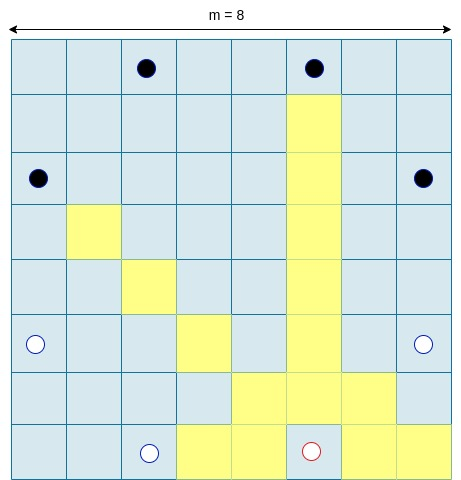
\includegraphics[width = 7cm, height = 6.6cm]{deplacement_qeen.jpeg}
                    \caption{Déplacements possibles}
                    \label{fig:deplacments possibles}
        \end{minipage}
            \hfill%
                \begin{minipage}[c]{.45\linewidth}
                      \centering
                    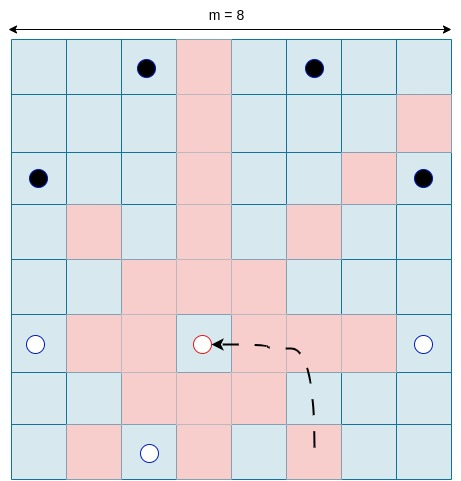
\includegraphics[width = 7cm, height = 6.6cm]{fleche_possibilites.jpeg}
                    \caption{Positions possibles de flèche}
                    \label{fig:fleches possibilites} 
                \end{minipage} 
            \end{figure}

        \subsection{Mise à jour des grilles de jeu}
        Après chaque tour dans le jeu, chaque joueur reçoit le mouvement effectué par son adversaire via le serveur, puis il l'applique sur son propre plateau de jeu en modifiant la position des reines adverses. Ensuite, le joueur choisit son propre mouvement pour le tour courant, l'applique sur son plateau de jeu et l'envoie au serveur pour être transmis à l'autre joueur. Il est important de noter que, étant donné que le serveur envoie toujours des copies des données entre les deux joueurs, la possibilité de tricher pour l'un des joueurs est exclue.
        \subsection{Fin d'une partie}
        La fin d'une partie est liée à possibilité d'effectuer un mouvement par un joueur, si un joueur est bloqué, c'est-à-dire toutes ces reines sont bloquées, alors il retourne comme mouvement le triple \textit{\{UINT\_MAX,UINT\_MAX,UINT\_MAX\}} qui est interprété par la fin de la partie par le serveur. La figure ~\ref{fig:gameover} montre un exemple de la fin d'une partie sur un graphe de largeur 8.
        \begin{figure}[h]
                \centering
                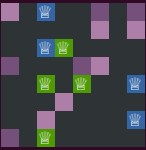
\includegraphics[height = 9cm, width = 10cm]{fin_de_la_partie.png}
                \caption{Le joueur vert a gagné la partie}
                \label{fig:gameover}
            \end{figure}
        \subsection{Gestion de la mémoire}
        
        La gestion de la mémoire est l'un des défis du projet. Pour bien gérer les allocations de mémoire dans la phase d'initialisation du jeu, la fonction $finalize$ de chaque joueur s'occupe de libérer la mémoire allouée pour le graphe du joueur et les tableaux des reines stockés pendant le jeu. En d'autres termes, la fin de la partie ne cause pas la libération de la mémoire, mais seulement la fin de la boucle de jeu. Pour d'autres fonctions, telles que $display$, qui utilisent également des allocations dynamiques en mémoire, on libère les blocs de mémoire alloués dès qu'on n'en a plus besoin dans le jeu. 
        \subsection{Boucle du jeu}
        Tout d'abord, pour commencer la boucle de jeu, il faut charger les joueurs dynamiquement à l’aide de la fonction \texttt{get\_opt} dans \texttt{server\_functions.c} et puis les initialiser chacun avec sa propre fonction d'initialisation. Ensuite, on initialise un graphe et on le crée deux copies, ainsi  que 3 copies de tableaux pour les positions initiales des reines, le premier pair sera utilisé par le serveur, les deux autres seront envoyés aux joueurs, afin que ceux\-ci ne puissent pas modifier les graphes appartenant au serveur ou à l'autre joueur, de plus le serveur choisit aléatoirement le joueur qui commence à l'aide de la fonction \textit{start\_player}.
        
        Au sein de cette boucle de jeu, chaque joueur envoie le mouvement qu'il a joué sous forme de \textit{struct move\_t}, le serveur fait la mise à jour de son graphe et après teste si la partie est terminée, sinon il passe le mouvement joué à l'autre jour qui est récupéré en utilisant la fonction \textit{next\_player}.
        
        À la fin de la partie, le serveur utilise les fonctions \textit{finalize} pour libérer l'espace mémoire utilisé par chaque joueur et aussi, il utilise la fonction \textit{free\_graph} pour libérer son propre graphe et il termine avec \texttt{dlclose} pour fermer les liens dynamiques entre le serveur et les clients.\\
        
    La boucle du jeu correspond au pseudo-algorithme suivant :
    \newpage
    \begin{algorithm}
    \caption{Boucle de jeu}
    \begin{algorithmic}
     \STATE move=\{-1,-1,-1\}
     \STATE player=star\_player()\\
    \For{ i=0, i \textless MAXTURNS }{
    \STATE move = player.play(move)
    \STATE execute\_move(move)
    \IF{is the game is finished }
    \STATE announce the player winner
    \STATE break
    \ENDIF
    \STATE player=next\_player()
    }
    \end{algorithmic}
    \end{algorithm}



    \section{Stratégies du jeu}
     Les joueurs doivent être automatisés et capables de jouer de manière autonome une fois initialisés. Ils doivent avoir leur propre stratégie et être en mesure de jouer des coups valides. De plus, ils doivent être adaptés leur propre graphe au cours de la partie afin de pouvoir retourner des coups valides. Enfin, lorsqu'une partie est terminée, ils doivent libérer le plateau de jeu et les allocations réalisées.
        \subsection{Stratégie de jeu aléatoire}
        À chaque tour de jeu, le joueur choisit une reine aléatoire et une direction aléatoire, si la reine peut se déplacer suivant la direction choisit, le joueur joue une case aléatoire parmi les destinations possibles, sinon il teste une autre direction, si la reine est bloquée, le joueur choisit une autre reine. Le joueur applique les mêmes étapes pour choisir la destination de sa flèche. La figure~\ref{fig:joueur_aleatoire} représente les étapes suivies par le client.
         \begin{figure}[h]
                \centering
                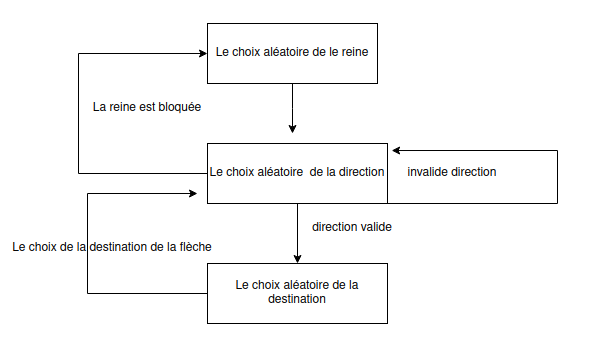
\includegraphics[scale=0.7]{jouer_aleato.png}
                \caption{Le choix de la destination pour la reine et la flèche }
                \label{fig:joueur_aleatoire}
            \end{figure}
            \newpage
        \subsection{Stratégie offensive}
        Bien que la stratégie consistant à prendre des positions au hasard peut être efficace dans certaines situations, une approche plus intentionnelle et délibérée est souvent nécessaire pour réussir dans un jeu. Afin d'améliorer nos chances de gagner, il est important de développer une stratégie solide qui prend en compte des facteurs tels que la disposition du plateau, les mouvements des autres joueurs et nos propres forces et faiblesses. Dans cet esprit, explorons un exemple de stratégie qui peut être mise en œuvre dans notre jeu de société programmé pour aider les joueurs à acquérir un avantage concurrentiel.\\
        la stratégie est similaire à celle de l'algorithme MiniMax, qui fonctionne en évaluant chaque coup possible pour chaque joueur jusqu'à un certain nombre de coups en avant, en utilisant une fonction d'évaluation pour mesurer l'avantage de chaque position, la seule différence est que nous nous arrêtons à le choix du premier coup,qui est la profondeur de l'arbre est égal à un. (Figure \ref{fig:tree }), avec $n$ le nombre des mouvement.
                         \begin{figure}[h]
                \centering
                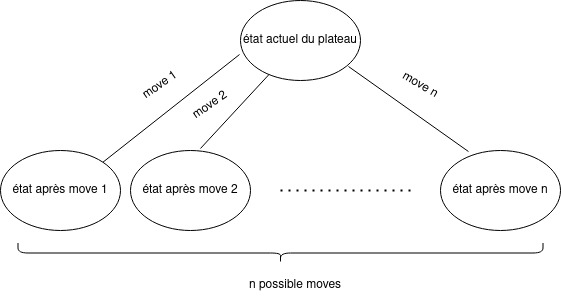
\includegraphics[scale=0.6]{tree.jpg}
                \caption{Arbre où chaque sommet est un état du jeu }
                \label{fig:tree }
            \end{figure}
            
        Pour faire un choix entre les coups l'heuristique suivant a été choisie
        \begin{equation*}
            H = N_{Current Player} - N_{Other Player} 
        \end{equation*}
        
        Avec $N_{joueur}$ le nombre total des positions voisines de toutes les reines du $joueur$, cette heuristique nous donne une assez bonne idée de la position préférable pour chaque joueur.
        
        Pour calculer l'heuristique, nous avons une fonction qui copie le graphe actuel et la position de ses reines, puis exécute le mouvement sur la copie, pour ensuite calculer l'heuristique de mouvement.
        Le problème avec ceci est que si nous ne limitons pas notre nombre de mouvements parmi lesquels choisir, nous aurions beaucoup de mouvements parmi lesquels choisir, cela signifie que nous aurons une complexité temporelle de $O(N_{moves})$ où $N_{moves}$ est le nombre de tous les mouvements possibles pour un joueur, qui dans les pires cas pourrait être très proche de $N_{v} \times N_{Q}$ avec $N_{v}$ et $N_{Q}$ sont le nombre de sommets et le nombre de reines. Si nous choisissons parmi ces positions, nous garantissons le blocage d'au moins une direction pour la reine ennemie. 
 % \\Il était important de limiter nos choix de mouvement.\\
 
        Pour faire un bon choix qui sélectionnera les mouvements qui ont une valeur heuristique plus élevée, la stratégie consiste à vérifier l'état du plateau à chaque tour. les positions prioritaires pour la reine et la flèche sont toutes les voisines des reines de l'autre joueur. La figure  \ref{fig:neighbors} le montre.
                 \begin{figure}[h]
                \centering
                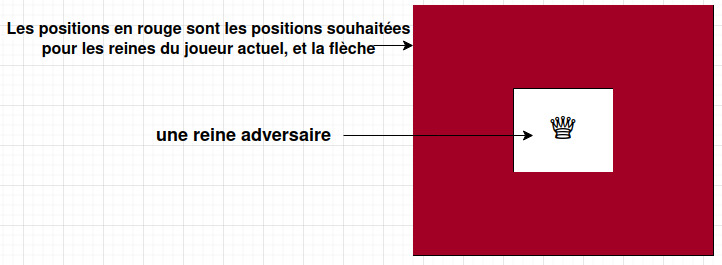
\includegraphics[width = 10cm, height = 4cm]{queen_neighbors.jpeg}
                \caption{Le choix préférable pour la reine et la flèche }
                \label{fig:neighbors}
            \end{figure}
  
 Il est possible de trouver des mouvements encore meilleurs, qui peuvent bloquer plus de degrés de liberté pour une pièce adverse, en un tour. Ce sont les positions voisines qui appartiennent à deux ou plusieurs reines adverses, cas de la figure \ref{fig:neighbors_pref}.
                  \begin{figure}[h]
                \centering
                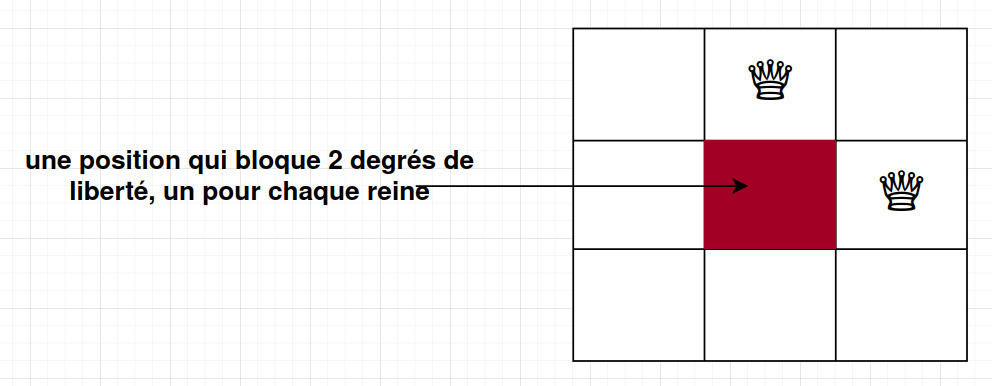
\includegraphics[scale=0.3]{strat.jpeg}
                \caption{Le choix préférable pour la reine et la flèche }
                \label{fig:neighbors_pref}
            \end{figure}

 
 En implémentant toutes les positions voisines de toutes les reines adverses sous la forme d'un tableau unidimensionnel, les positions qui bloquent le plus de dégrée de libertés auraient l'occurrence la plus élevée dans cette liste.
 Au final nous avons réduit nos choix de mouvements en choisissant le mouvement de cette liste.
 
        \subsection{Stratégie défensive}
        La deuxième stratégie consiste à diviser le processus en deux phases distinctes. La première phase, appelée phase d'ouverture, est mise en œuvre lorsque le nombre de tours est inférieur au nombre de reines. Son objectif est de déplacer toutes les reines vers des positions qui ne se trouvent pas sur les côtés de la grille, afin de leur offrir une plus grande liberté de mouvement lors des prochains déplacements.
         \begin{figure}[h]
                \centering
                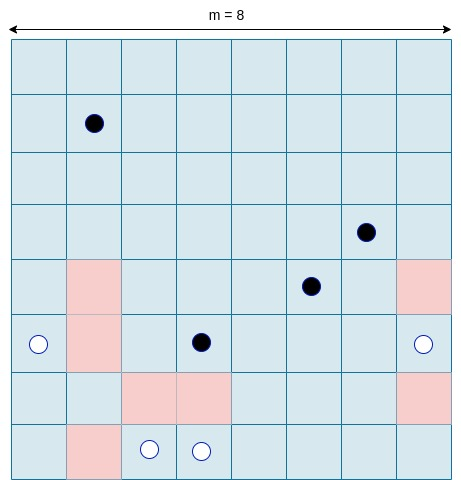
\includegraphics[scale=0.3]{strategy_oppening.jpeg}
                \caption{La grille après la phase d'ouverture.}
                \label{fig:opening}
            \end{figure}

Une fois la phase d'ouverture terminée, la deuxième phase est initiée. Dans cette phase, nous avons deux choix possibles pour déplacer les reines. Le premier choix consiste à les déplacer vers des positions offrant un degré de liberté plus élevé, c'est-à-dire des positions où il y a plus de cases libres. Cela augmente les possibilités de réussite. Si aucune position de ce type n'est disponible, nous procédons de manière aléatoire en déplaçant la reine vers n'importe quelle position possible.

Une fois que la destination de la reine a été choisie soit dans la phase d'ouverture où dans la deuxième phase, nous cherchons ensuite un emplacement où placer un bloc. L'objectif est de bloquer les reines adverses, donc nous cherchons une reine qui a le moins de voisins possible, afin de la bloquer efficacement. Si notre reine ne peut pas atteindre une telle position, nous choisissons aléatoirement un emplacement pour notre bloc.
\begin{figure}[h]
                \centering
                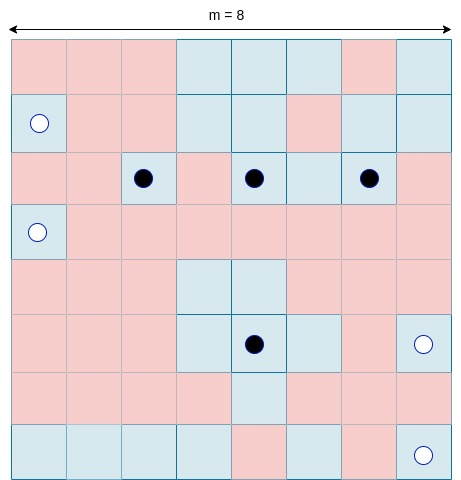
\includegraphics[scale=0.3]{strategy_endings.jpeg}
                \caption{La fin du jeu.}
                \label{fig:ending}
            \end{figure}
    \section{Affichage du jeu}
        Pour pouvoir visualiser l'avancement des parties, nous avons réalisé deux affichages, le premier est un affichage sur le terminal en utilisant les codes pour l'affichage des couleurs en langage C, l'autre affichage est un affichage en utilisant \textbf{sdl}, la figure \ref{fig:display} montre les deux affichages réaliser pour visualiser les parties.
        \begin{figure}[h]
    \centering
    \vspace{.5cm}
    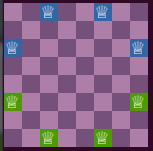
\includegraphics[scale=0.85]{affichage_terminal.png}\quad
    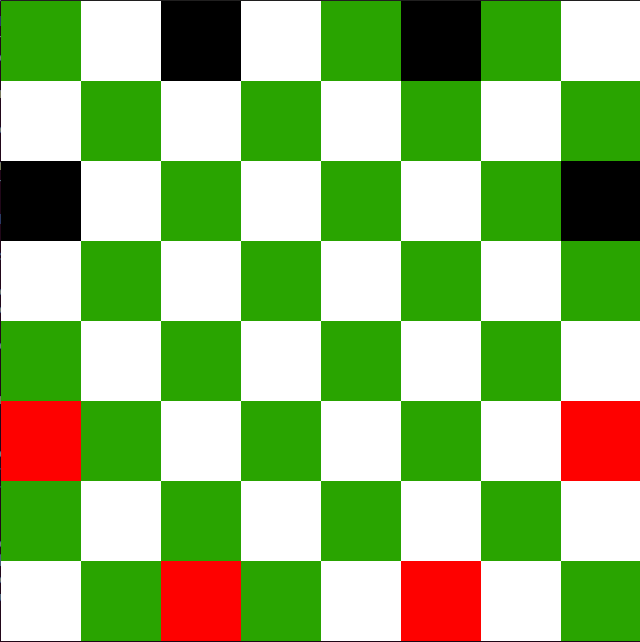
\includegraphics[scale=0.2]{affichage_sdl.png}
    \caption{L'affichage terminal et l'affichage sdl }
    \label{fig:display}
\end{figure}\\
    \section{Tests}
    Afin de juger la fonctionnalité de nos fonctions, plusieurs tests de nos fonctions ont été réalisés, en utilisant la bibliothèque "assert" en C et en vérifiant la couverture avec "gcov".\\
    
        \subsection{Tests structurels}
Les tests structurels, sont des tests qui évaluent la structure interne du programme. Ils sont conçus pour identifier les erreurs de codage, les bogues. Nous avons utilisé différents outils pour effectuer des tests structurels dans notre projet, notamment gdb, valgrind et gcov. gdb est un outil de débogage qui nous a permis d'exécuter le programme pas à pas et d'identifier les erreurs de codage en temps réel. Valgrind est un outil de détection de fuites de mémoire qui nous a aidés à identifier les fuites de mémoire et les erreurs d'allocation de mémoire dans notre programme. Enfin, gcov est un outil de profilage de code qui nous a permis d'analyser la couverture de code et d'identifier les parties du code qui n'ont pas été exécutées pendant les tests. L'utilisation combinée de ces outils nous a permis d'identifier et de corriger les erreurs de codage, de garantir une utilisation correcte de la mémoire et d'augmenter la couverture de code testée, ce qui a contribué à améliorer la qualité et la fiabilité de notre programme.
        \subsection{Tests fonctionnels}
        Les tests fonctionnels sont censés vérifier que le programme fonctionne conformément aux spécifications, aux exigences et à nos attentes, qui sont les suivants: 
        \begin{itemize}
    \item Test d'initialisation du graphe en diffèrent position (classique, donut ....). Nous initialisons un graphe avec 25 sommets puis nous vérifions la valeur dans sa matrice d'adjacence pour chaque sommet spécifique, et pour chaque type de graphe. 
    \item  Tests des fonctions de mouvement.
qui inclut les fonctions qui vérifient les mouvements possibles ainsi que les fonctions qui exécutent le mouvement.
\end{itemize}
\subsection{Tests de nos stratégies}

Afin de vérifier l'efficacité de nos stratégies, nous avons décidé de créer un script shell qui prend en paramètre les résultats de l'exécution de notre programme. Nous avons modifié ce dernier pour qu'il renvoie soit 0, soit 1 en fonction du joueur gagnant. Ce script exécute notre programme un nombre prédéfini de fois (par exemple, 100, 1000 ou 10000) avec différentes tailles de jeu. Plus la taille est grande et le nombre de matchs est élevé, plus nous obtenons des résultats précis.

Ensuite, nous calculons la probabilité qu'un joueur gagne en comptant le nombre de 0 (respectivement de 1) pour chaque joueur et en le divisant par le nombre total de matchs joués. Ce script nous permet de mesurer l'efficacité de nos stratégies, en particulier face à un joueur aléatoire. Nous avons ainsi pu atteindre une probabilité de victoire de nos joueurs supérieure à 80\%.

% \lstset{language=bash}

% \begin{lstlisting}
% #!/bin/bash
% total_games=1000
% black_count_0=0
% white_count_1=0
% for ((i=0; i<total_games; i++)); do
%     result=$(./server libplayer1.so libplayer2.so -m 8 -s 150)   par le nom ou le chemin vers votre programme
%     if [ "$result" == "0" ]; then
%         ((black_count_0++))
%     elif [ "$result" == "1" ]; then
%         ((white_count_1++))
%     fi
% done
% prob_0=$(bc <<< "scale=4; $black_count_0 / $total_games")
% prob_1=$(bc <<< "scale=4; $white_count_1 / $total_games")
% echo "The probability that black_player wins: $prob_0"
% echo "The probability that white_player wins: $prob_1"
% \end{lstlisting}

En résumé, nous avons utilisé un script shell pour évaluer l'efficacité de nos stratégies en effectuant un grand nombre de matchs avec différentes tailles de jeu. 
    \section{Améliorations possibles}
        \subsection{Utilisation de l'algorithme Alpha-beta}
dans notre algorithme offensif, nous n'avons vérifié que l'heuristique pour les prochains mouvements, nous n'avons pas été jusqu'au bout avec l'algorithme minimax implémentant la structure arborescente à une profondeur plus élevée, et même avec cela, la complexité de l'algorithme serait à peu près exponentielle en fonction de la profondeur de l'arbre des mouvements.
\\L'algorithme pourrait être optimisé en utilisant la méthode alpha-beta, qui accélère la recherche du meilleur mouvement dans l'arbre, en éliminant les branches des mouvements qui ne seront pas sélectionnées


\subsection{Intelligence artificielle}

Une amélioration possible d'une implémentation de jeu avec l'intelligence artificielle (IA) basée sur le machine learning serait de rendre l'IA plus adaptative et dynamique. Plutôt que de simplement programmer des règles et des comportements préétablis pour l'IA, une implémentation de machine learning permettrait à l'IA de s'adapter et d'apprendre en temps réel en fonction des actions du joueur et des résultats de ses propres actions. Par exemple, dans un jeu de stratégie en temps réel, l'IA pourrait apprendre à anticiper les mouvements du joueur et à adapter ses propres stratégies en fonction des résultats de ses actions précédentes. Cela rendrait le jeu plus dynamique et offrirait une expérience de jeu plus immersive pour le joueur. En outre, cela permettrait également à l'IA de s'améliorer et de devenir plus efficace au fil du temps, ce qui augmenterait le défi et l'intérêt pour le joueur.

    \section{Conclusion}
En résumé, notre projet de programmation sur le jeu "Les Amazones" a été une expérience stimulante qui nous a permis de mettre en pratique nos compétences en programmation impérative. Malgré les obstacles rencontrés, nous avons su trouver des solutions alternatives et améliorer notre compréhension. La collaboration en équipe a été essentielle, nous permettant d'échanger des idées et de résoudre efficacement les problèmes. L'utilisation d'outils de débogage tels que GDB et Valgrind a renforcé la qualité de notre code, tandis que la manipulation de librairies et la mise en place d'un serveur nous ont exposés à des concepts avancés de programmation. Dans l'ensemble, ce projet a été un jalon significatif dans notre parcours de développement, nous préparant mieux à relever les futurs défis en programmation.

\end{document}
